\documentclass[10pt,a4paper]{article}
\usepackage[margin=2cm]{geometry}
\usepackage{amsmath,amssymb,booktabs,graphicx,float,caption,tikz,xcolor}
\usepackage[hidelinks]{hyperref}
\usetikzlibrary{arrows.meta,positioning,shapes.geometric}
\graphicspath{{../../results/figures/}}
\captionsetup{font=small,labelfont=bf}
\setlength{\parskip}{4pt}\setlength{\parindent}{0pt}
\newcommand{\tablein}[1]{\input{tables/#1.tex}}
\tikzset{box/.style={draw,rounded corners,fill=blue!6,minimum height=7mm,align=center,font=\small},arr/.style={-{Stealth},thick}}

\title{Restoring Visibility Through Haze, Water, Glass and Plastic\\\large Classical (non-learning) restoration with the Dark Channel Prior as baseline --- detailed report}
\author{Shaik Areesh (2026909008), Noel Alex Jacob (2025201085), Sri Harshit K (2024102022)\\ DIP (CS7.404), IIIT Hyderabad}
\date{Draft of 2026-11-04 --- presentation 2026-11-12}

\begin{document}
\maketitle
\tableofcontents

\section{Objective and what was built}
The question: how well do classical image-processing tools (spatial filters, histogram methods, frequency-domain filters, priors) restore a picture seen through four media --- \emph{haze}, \emph{turbid water}, \emph{glass} (fog, dirt, droplets) and \emph{translucent plastic} --- and does anything beat the Dark Channel Prior (DCP) baseline? No learned model is used.

We built (all code in \texttt{code/}, results reproducible, every number in this report is read from \texttt{results/tables/} by \texttt{make\_report\_tables.py}):
\begin{itemize}
\item forward models (synthesisers) for each medium, with stacking of layers, and a drag-and-drop HTML demo (\texttt{demo/}) that uses the same models and random generator;
\item 40 restoration methods plus a step-sequence search (any ordered chain of up to three methods);
\item metrics: PSNR, SSIM, CIEDE2000, entropy, contrast, UCIQE, dark channel, colour cast, and agreement scores between rankings;
\item experiments: matched synthetic pairs, real pairs, parameter and severity sweeps, step-order search with held-out verification, synthetic-versus-real checks, model calibration, a frequency-domain study with haze removal by subtraction, failure analysis and stacked media.
\end{itemize}

\section{Data}
\small\begin{tabular}{p{3.4cm}p{6.4cm}p{6cm}}\toprule
Source & What & Use\\\midrule
NYU Depth v2 (indoor) & clear pictures with depth & 288 matched synthetic pairs for haze, water, glass, plastic\\
O-HAZE, I-HAZE, Dense-Haze, NH-Haze, RESIDE-SOTS & real hazy/clear pairs (185 pairs in the real stage) & real haze\\
RainDrop (Qian et al.) & real raindrops on glass with clean pane (58 pairs) & real glass\\
UIEB & real underwater pictures (references only) & looked at, not scored (no true clear reference)\\
Own captures & water, glass fog/dirt, plastic, stacks & \emph{pending} --- no public plastic data exists\\\bottomrule
\end{tabular}

\section{Forward models and their equations}
Full derivations (spatial and frequency domain, with the literature check) are in \texttt{docs/model-equations.md}. The shared idea: a medium \emph{keeps a fraction} $t$ of the scene light and \emph{adds} light $A(1-t)$.
\begin{align}
\text{haze:}\quad & I = J\,t + A(1-t),\quad t = e^{-\beta d(x)}\\
\text{water:}\quad & I_c = J_c\,e^{-\beta_c d} + B_c(1-e^{-\beta_c d}),\quad \beta_R>\beta_G>\beta_B\\
\text{glass droplets:}\quad & I = (1-w)J + w\,(0.9\,g_\sigma{*}J + 0.1A)\\
\text{plastic:}\quad & I = t\,\kappa\,(h_\sigma{*}J)+A(1-t)\\
\text{stack:}\quad & I_2 = t_1t_2J + t_2A_1(1-t_1) + A_2(1-t_2)
\end{align}
In the frequency domain (spectral ratio $R(f)=|\hat I|/|\hat J|$): haze $R=t$ (veil only at $f=0$); plastic $R=t\kappa e^{-2\pi^2\sigma^2f^2}$; water $R_c=t_c$; a stack multiplies the ratios. Table~\ref{tab:theory} shows measured against predicted values.
\begin{table}[H]\centering\tiny\tablein{theory_checks}\caption{Frequency-domain theory against measurement on our synthetic pictures and real data (rms error of the predicted curve; mid-band ratio measured and predicted).}\label{tab:theory}\end{table}

\section{Restoration pipelines}
\begin{figure}[H]\centering
\resizebox{\textwidth}{!}{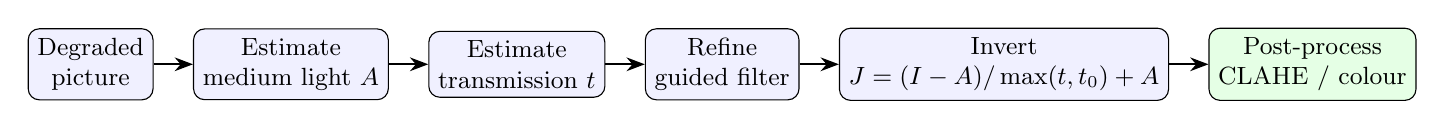
\begin{tikzpicture}[node distance=5mm]
\node[box](a){Degraded\\picture};
\node[box,right=of a](b){Estimate\\medium light $A$};
\node[box,right=of b](c){Estimate\\transmission $t$};
\node[box,right=of c](d){Refine\\guided filter};
\node[box,right=of d](e){Invert\\$J=(I-A)/\max(t,t_0)+A$};
\node[box,right=of e,fill=green!10](f){Post-process\\CLAHE / colour};
\foreach \x/\y in {a/b,b/c,c/d,d/e,e/f}{\draw[arr](\x)--(\y);}
\end{tikzpicture}}
\caption{The DCP pipeline (baseline). Medium-aware variants change the airlight and transmission steps (UDCP uses only green and blue; local airlight; near-global $t$).}\end{figure}
The sequence search treats any of the 40 methods as a step: all 259 chains of length $\le3$ drawn from a candidate list are scored on search set A and the best chain is verified on a disjoint set B (order matters by up to 3.1 dB).

\section{Results}
Unless stated, synthetic results use the \emph{calibrated} presets (haze and glass fitted to real pictures; section~\ref{sec:ba}). The runs with the original hand-chosen presets are kept in \texttt{results\_original\_presets/} and compared in section~\ref{sec:ba}.
\subsection{Matched synthetic pairs (all severities pooled)}
\begin{table}[H]\centering\scriptsize
\begin{minipage}{.48\textwidth}\centering\textbf{haze}\\\tablein{matched_haze}\end{minipage}\hfill
\begin{minipage}{.48\textwidth}\centering\textbf{water}\\\tablein{matched_water}\end{minipage}\\[6pt]
\begin{minipage}{.48\textwidth}\centering\textbf{glass}\\\tablein{matched_glass}\end{minipage}\hfill
\begin{minipage}{.48\textwidth}\centering\textbf{plastic}\\\tablein{matched_plastic}\end{minipage}
\caption{Best methods per medium on matched synthetic pairs (calibrated haze and glass; water and plastic identical to the original run).}\end{table}
\begin{figure}[H]\centering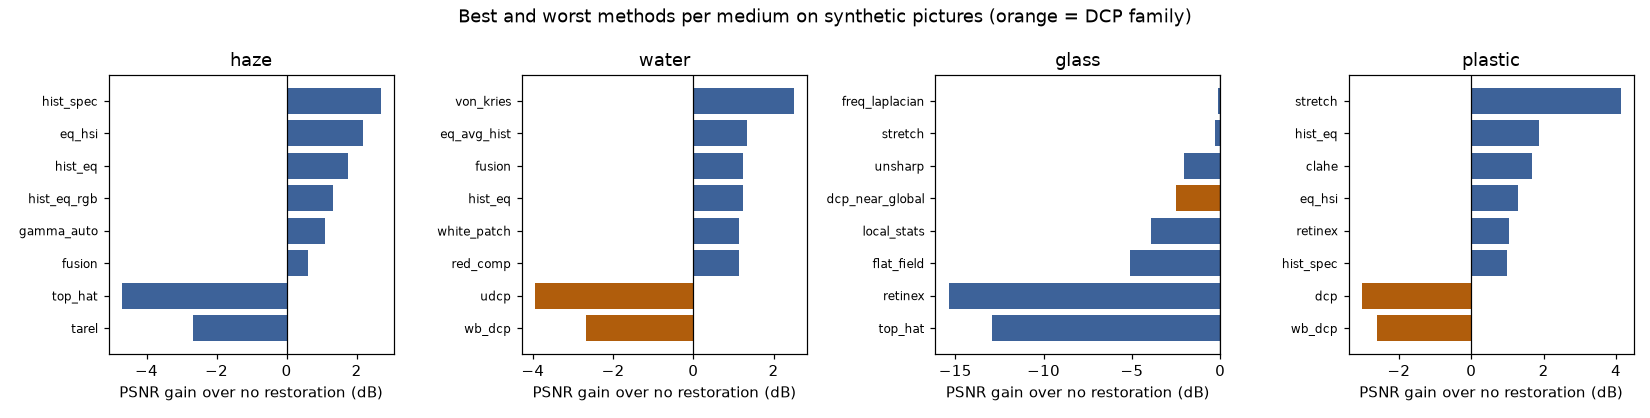
\includegraphics[width=\textwidth]{report_gain_over_none.png}\caption{Gain over no restoration, per method and medium.}\end{figure}
\begin{figure}[H]\centering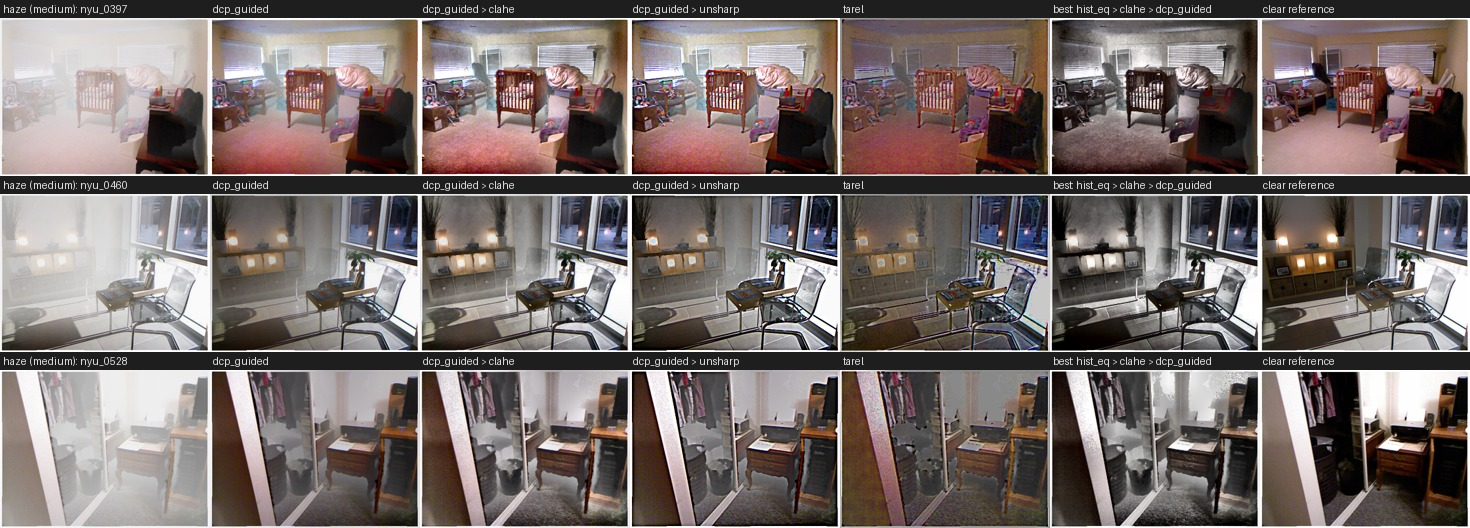
\includegraphics[width=.9\textwidth]{report_ba_haze.jpg}\caption{Before and after, synthetic haze: degraded, restored by several methods, clear reference.}\end{figure}
\begin{figure}[H]\centering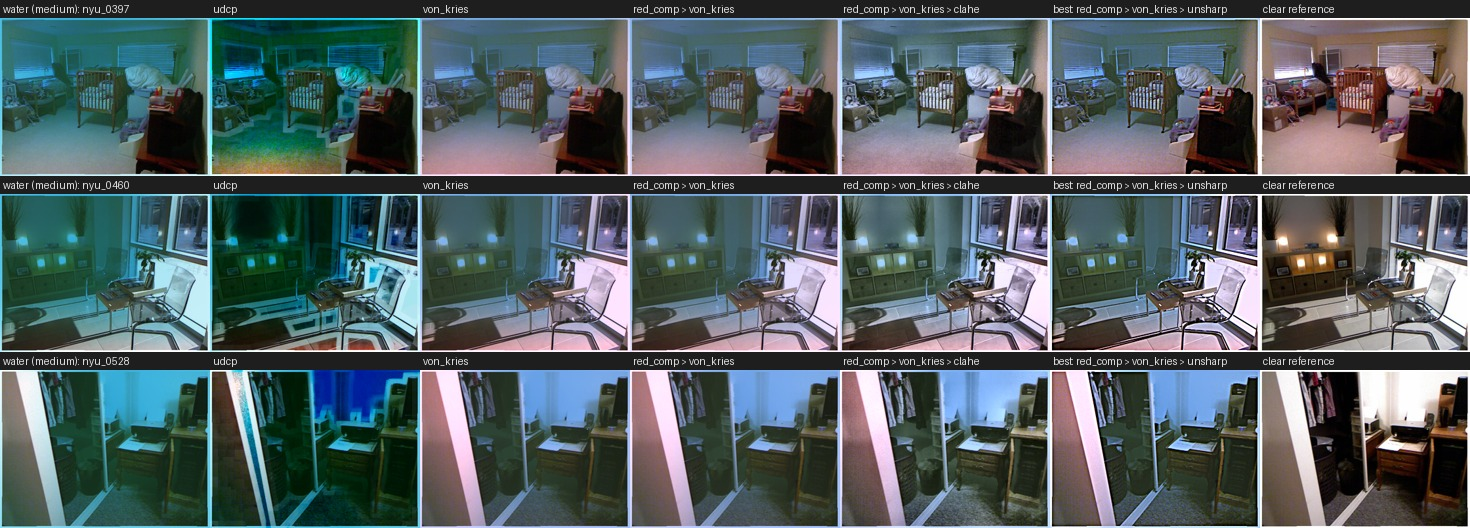
\includegraphics[width=.9\textwidth]{report_ba_water.jpg}\caption{Before and after, synthetic water.}\end{figure}
\begin{figure}[H]\centering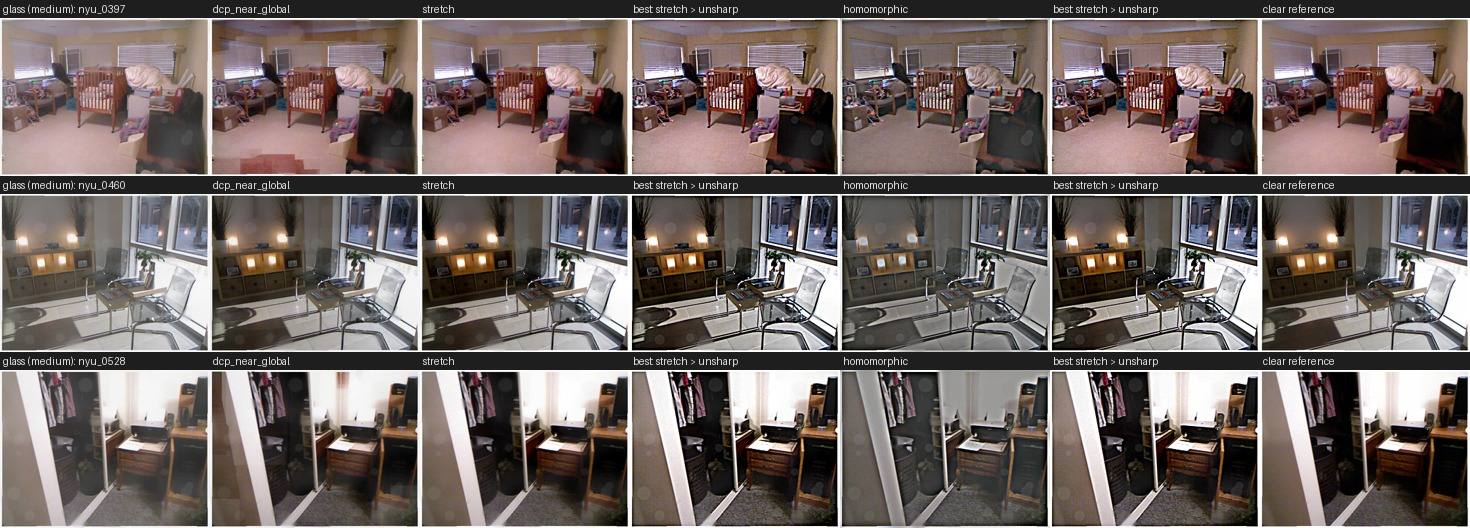
\includegraphics[width=.9\textwidth]{report_ba_glass.jpg}\caption{Before and after, synthetic glass.}\end{figure}
\begin{figure}[H]\centering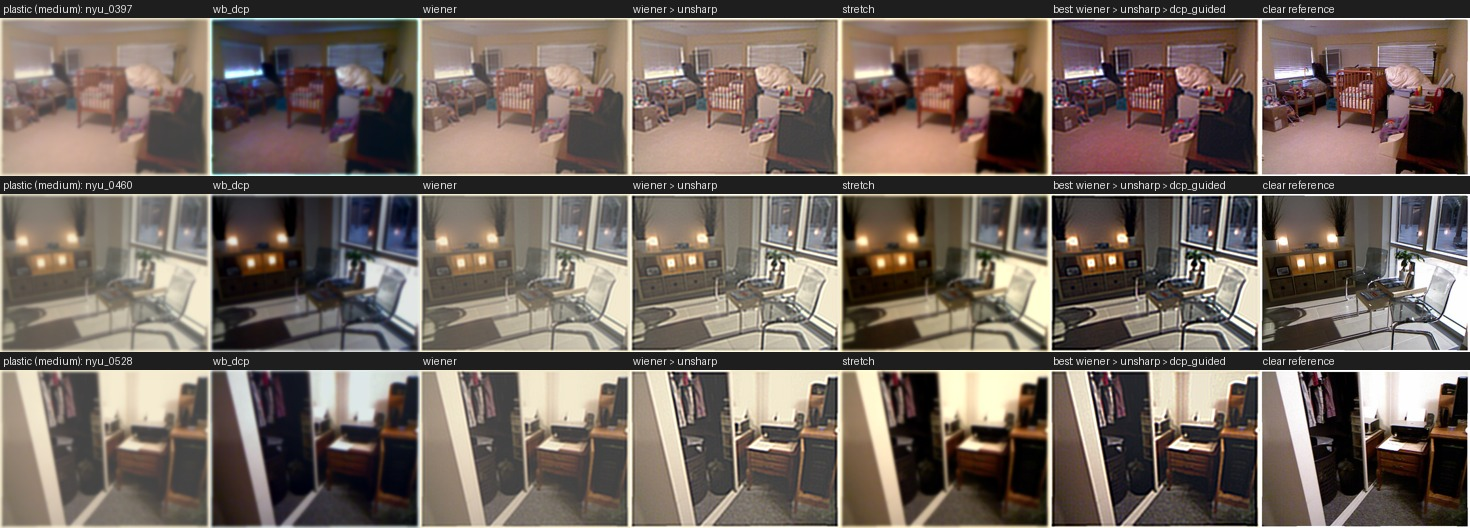
\includegraphics[width=.9\textwidth]{report_ba_plastic.jpg}\caption{Before and after, synthetic plastic.}\end{figure}
\begin{figure}[H]\centering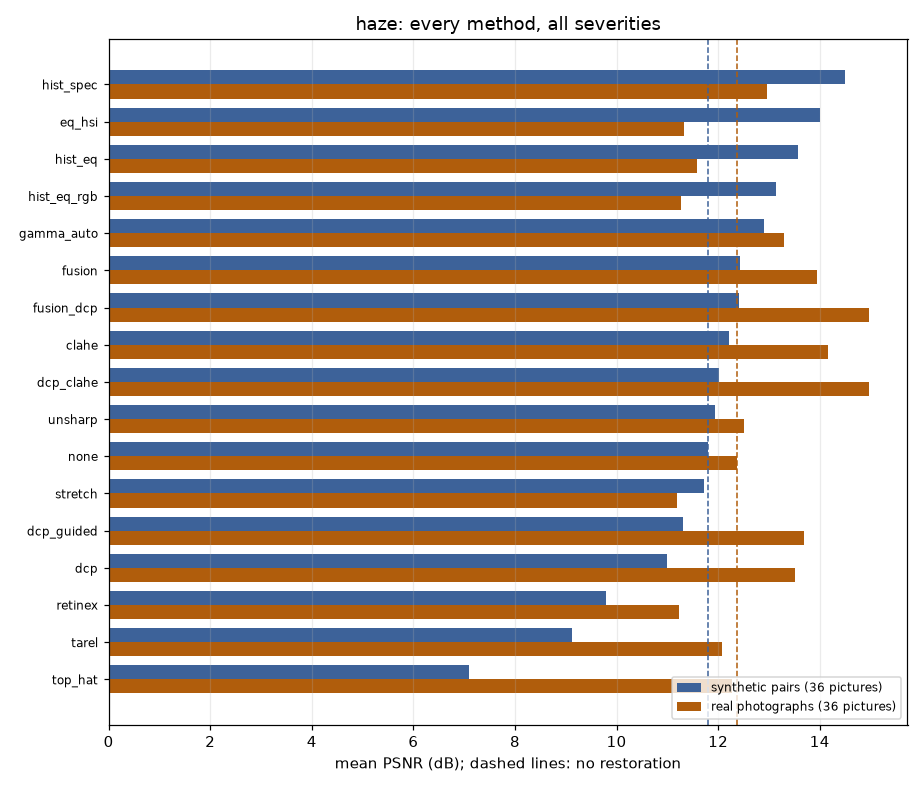
\includegraphics[width=.75\textwidth]{report_methods_haze.png}\caption{Method comparison, synthetic haze.}\end{figure}
\begin{figure}[H]\centering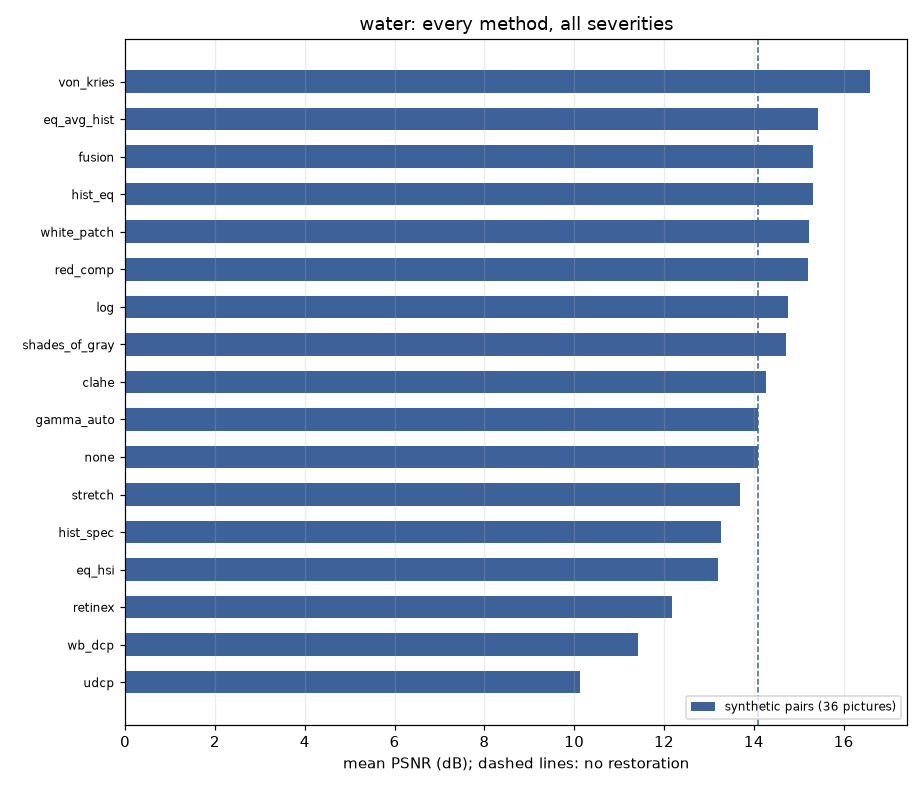
\includegraphics[width=.75\textwidth]{report_methods_water.png}\caption{Method comparison, synthetic water.}\end{figure}
\begin{figure}[H]\centering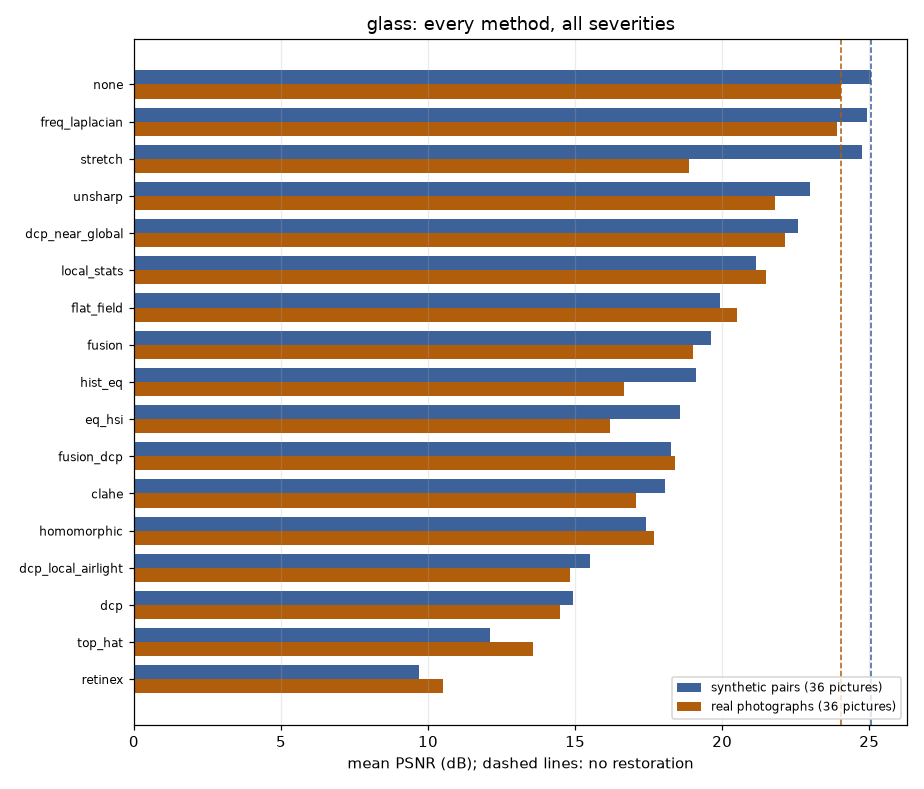
\includegraphics[width=.75\textwidth]{report_methods_glass.png}\caption{Method comparison, synthetic glass.}\end{figure}
\begin{figure}[H]\centering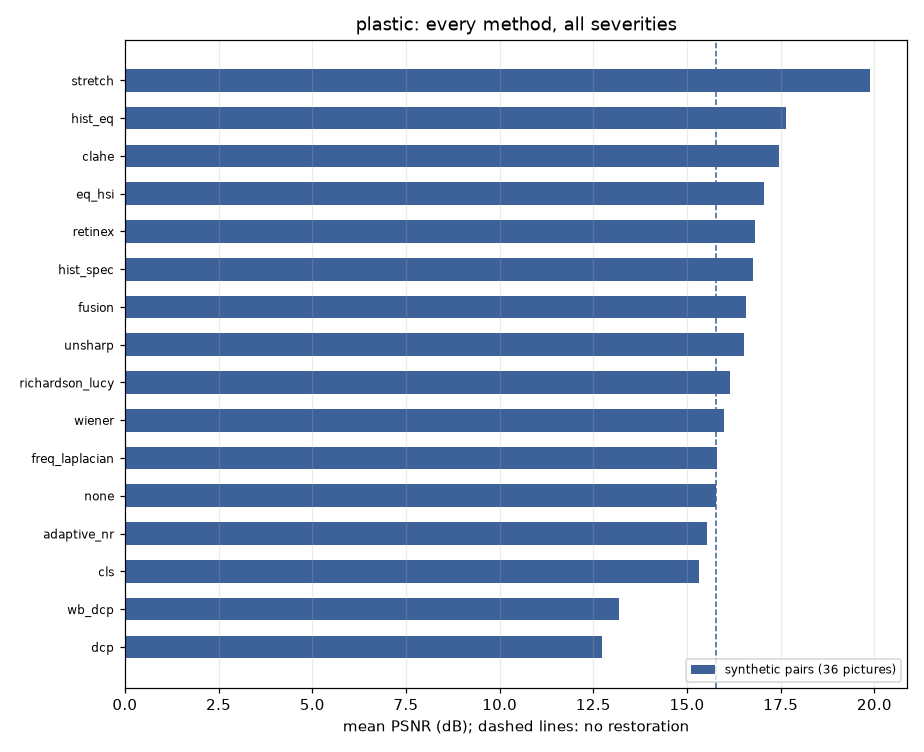
\includegraphics[width=.75\textwidth]{report_methods_plastic.png}\caption{Method comparison, synthetic plastic.}\end{figure}

\subsection{Real pictures}
\begin{table}[H]\centering\scriptsize
\begin{minipage}{.48\textwidth}\centering\textbf{real haze (185 pairs)}\\\tablein{real_haze}\end{minipage}\hfill
\begin{minipage}{.48\textwidth}\centering\textbf{real raindrops on glass}\\\tablein{real_glass}\end{minipage}
\caption{Real data. On real haze a contrast step after DCP (CLAHE) beats DCP alone; on raindrops nothing helps.}\end{table}
\begin{figure}[H]\centering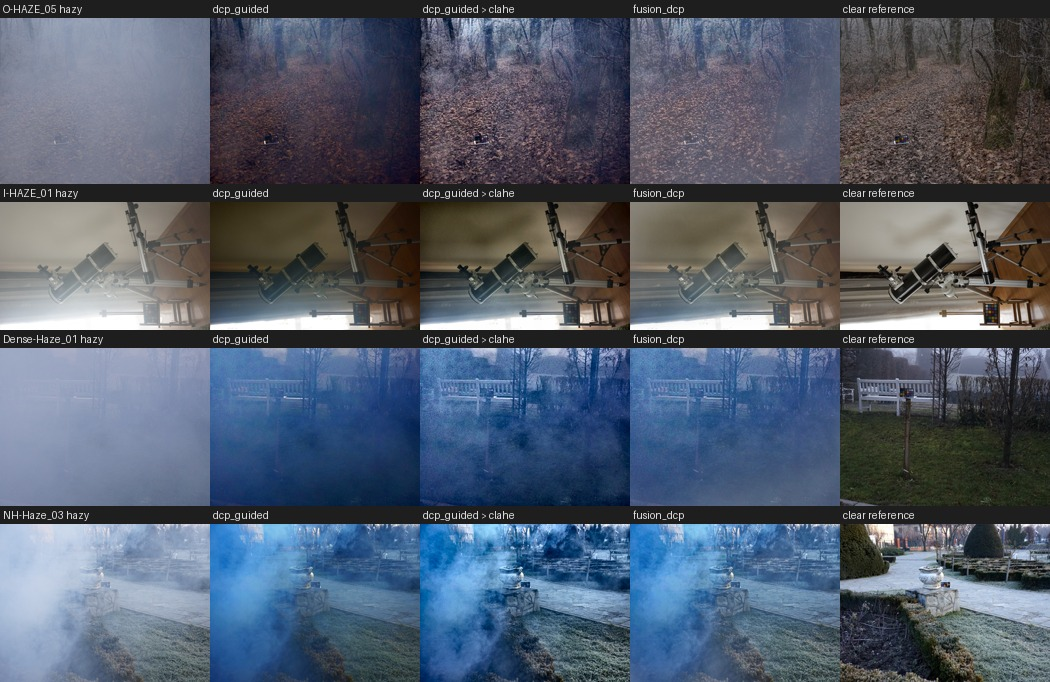
\includegraphics[width=.95\textwidth]{report_ba_real_haze.jpg}\caption{Real haze, before and after: DCP leaves a blue cast and a dark picture; adding CLAHE or fusion recovers brightness and detail.}\end{figure}
\begin{figure}[H]\centering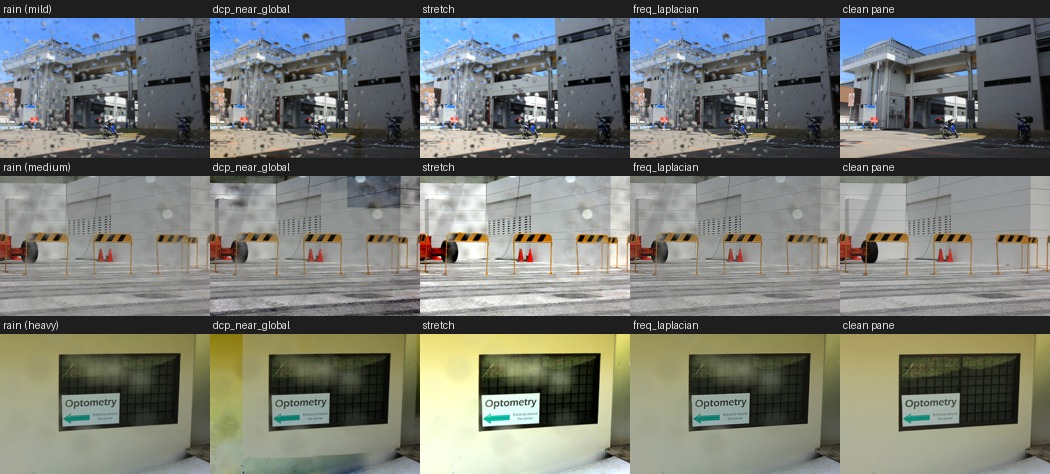
\includegraphics[width=.95\textwidth]{report_ba_real_glass.jpg}\caption{Real raindrops, before and after.}\end{figure}

\subsection{Step order and post-processing}
\begin{table}[H]\centering\scriptsize\tablein{pipelines_verify}\caption{Best searched chain per medium, verified on held-out pictures, against DCP alone and nothing. With calibrated haze a contrast chain before DCP beats DCP alone (13.66 against 12.86 dB); with the original haze nothing did. On real haze DCP$\to$CLAHE gains +1.28 dB over DCP (SE 0.22; better on 29 of 36 pairs, SSIM +0.092). On calibrated glass the best chain is doing nothing.}\end{table}
\begin{figure}[H]\centering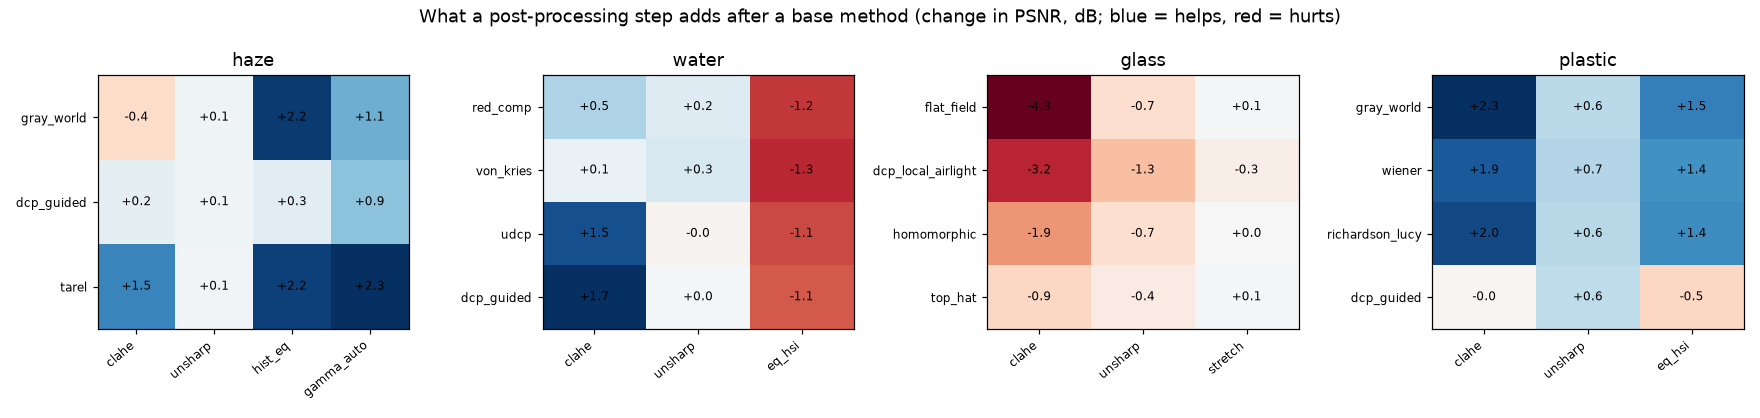
\includegraphics[width=\textwidth]{report_postprocessing.png}\caption{What a post-processing step adds after a base method (change in PSNR). Histogram equalisation after gray-world helps haze (+3.8 dB) but hurts after DCP (-1.5 dB): post-processing is not free.}\end{figure}
\begin{figure}[H]\centering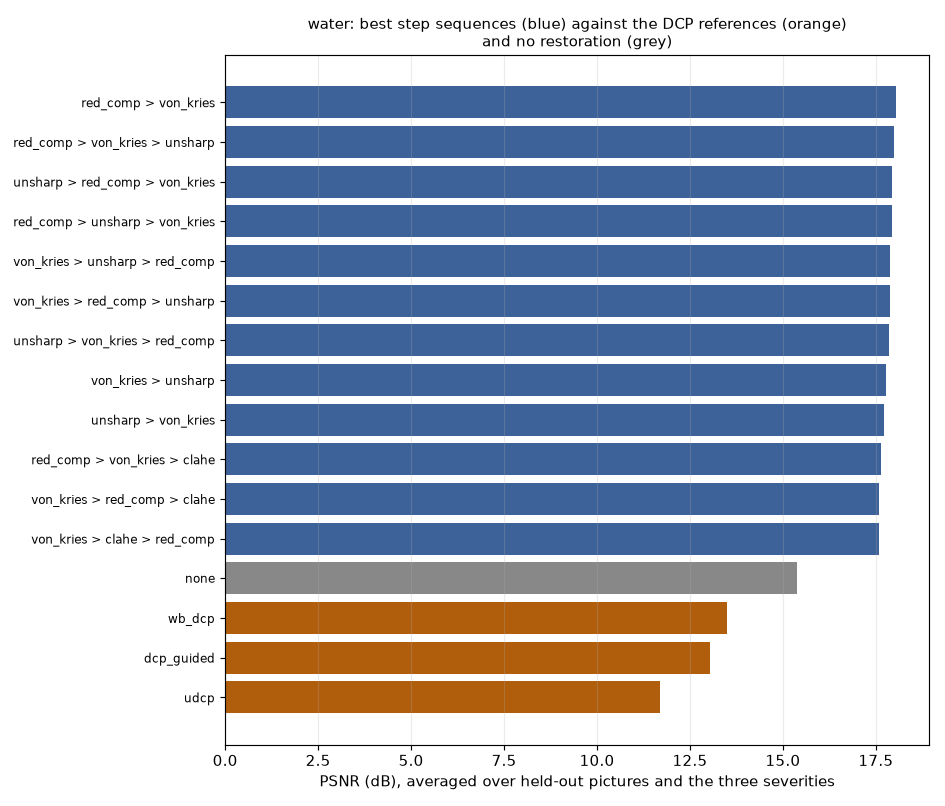
\includegraphics[width=.49\textwidth]{pipelines_water.png}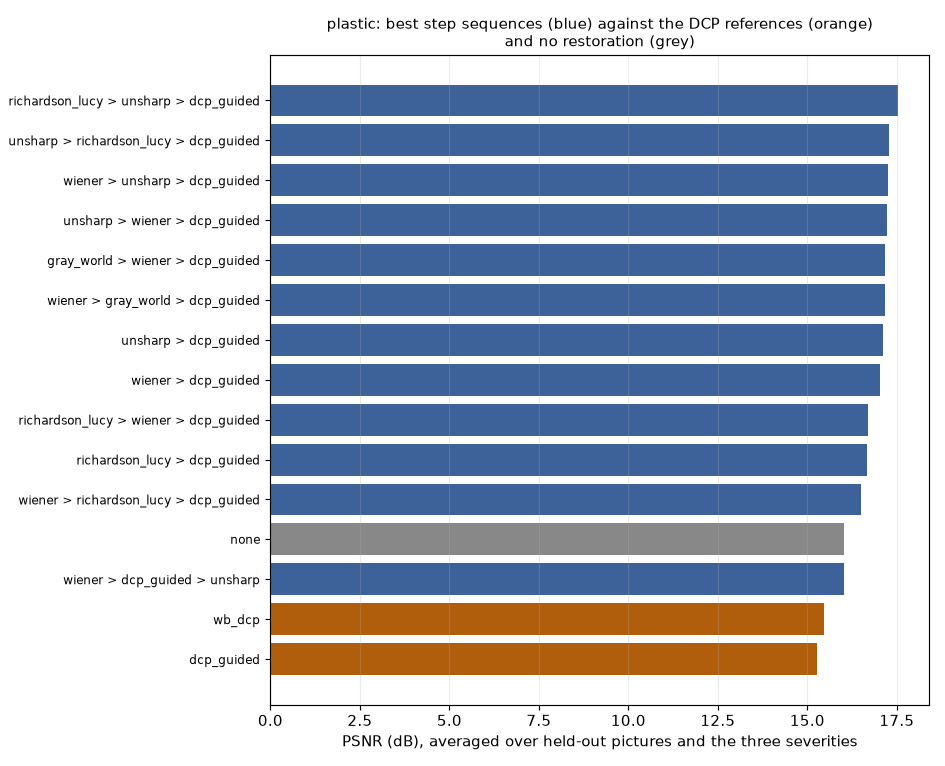
\includegraphics[width=.49\textwidth]{pipelines_plastic.png}\caption{Searched sequences: water (red compensation, von Kries, unsharp: +4.5 dB over DCP) and plastic (Wiener, unsharp, DCP: +1.8 dB).}\end{figure}

\subsection{Parameter and severity sweeps}
\begin{figure}[H]\centering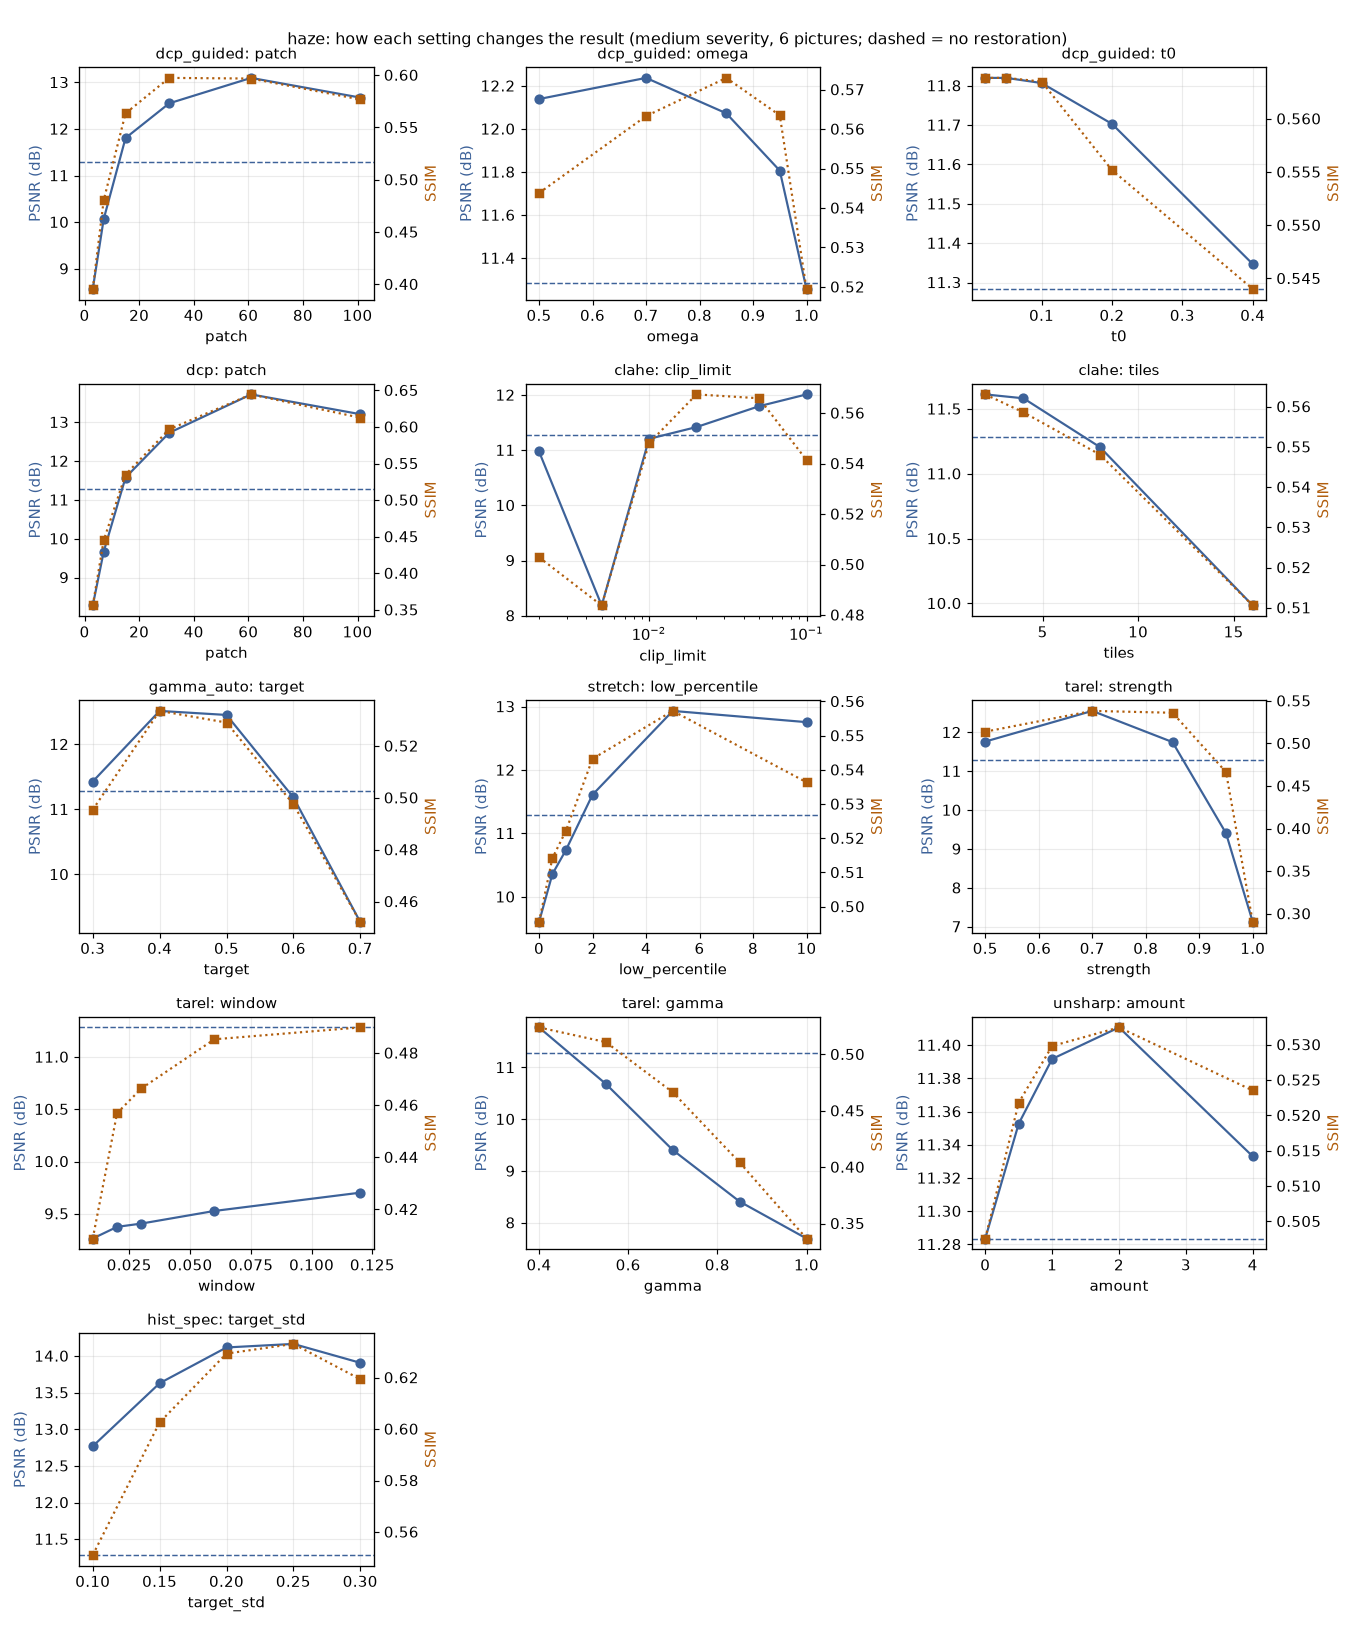
\includegraphics[width=.49\textwidth]{sweeps_haze.png}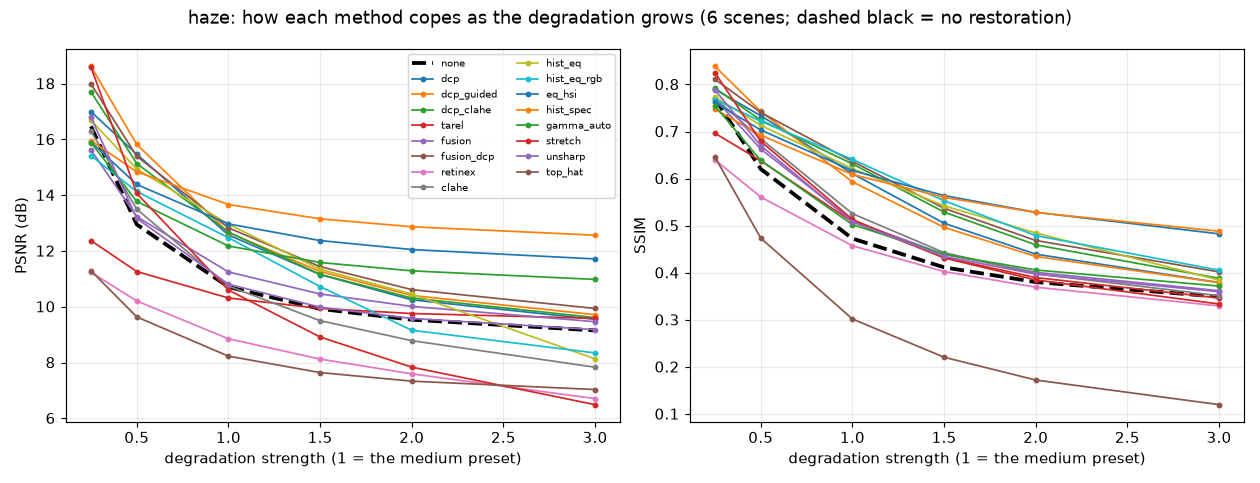
\includegraphics[width=.49\textwidth]{severity_haze.png}\caption{Left: parameter spread for haze methods. Right: severity sweep for haze with the calibrated model. (The 9.7 dB spread and the Tarel-over-DCP crossing quoted in the log were measured with the original presets; see the frozen before-results.)}\end{figure}
\begin{figure}[H]\centering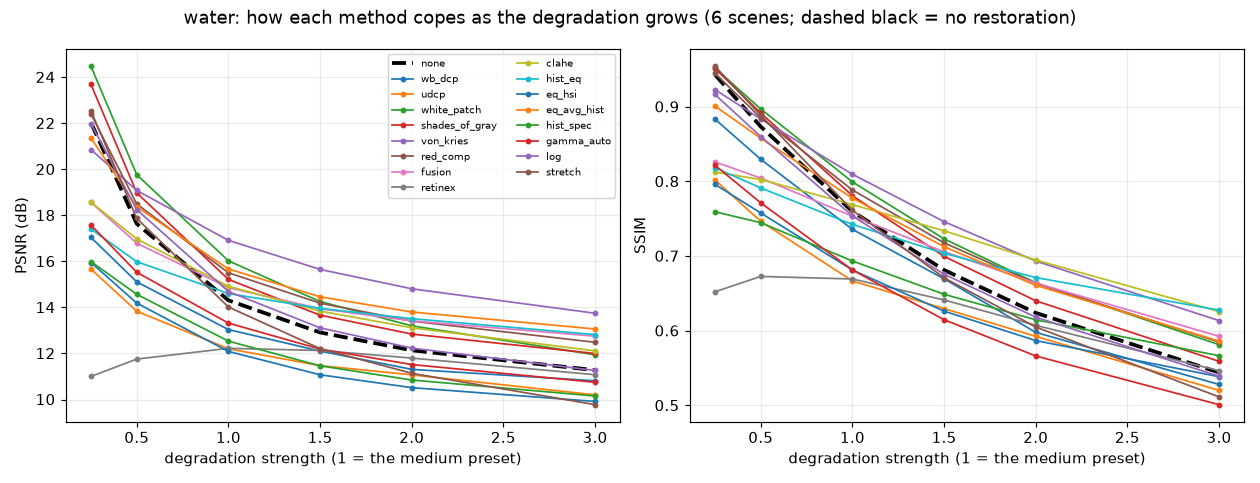
\includegraphics[width=.49\textwidth]{severity_water.png}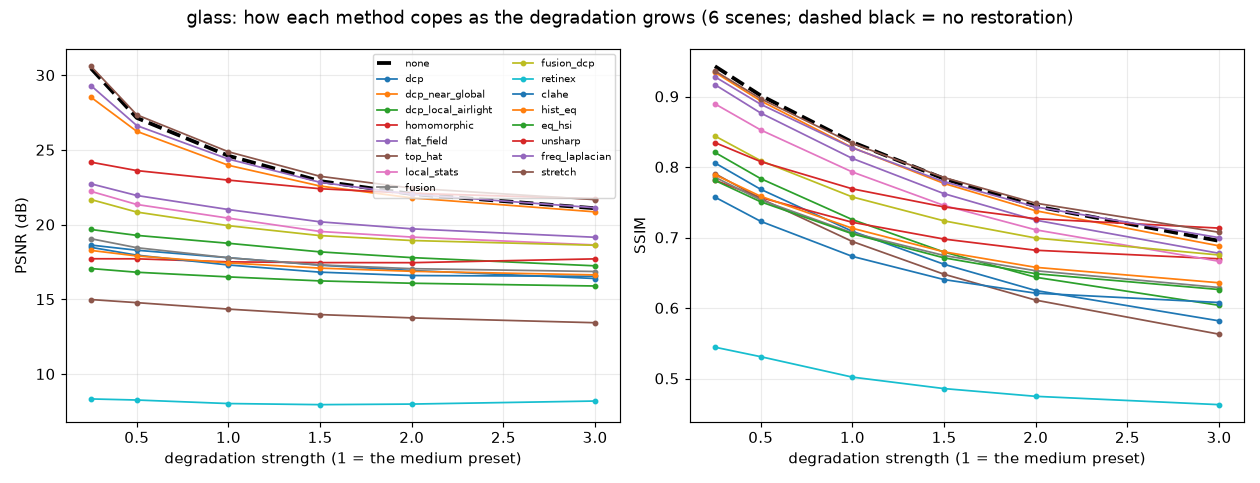
\includegraphics[width=.49\textwidth]{severity_glass.png}\caption{Severity sweeps, water and glass.}\end{figure}

\subsection{Do the synthetic models match real pictures?}
\begin{table}[H]\centering\scriptsize\tablein{ranking_agreement}\caption{Do methods rank the same on synthetic and real data? Rank correlation of method scores.}\end{table}
\begin{figure}[H]\centering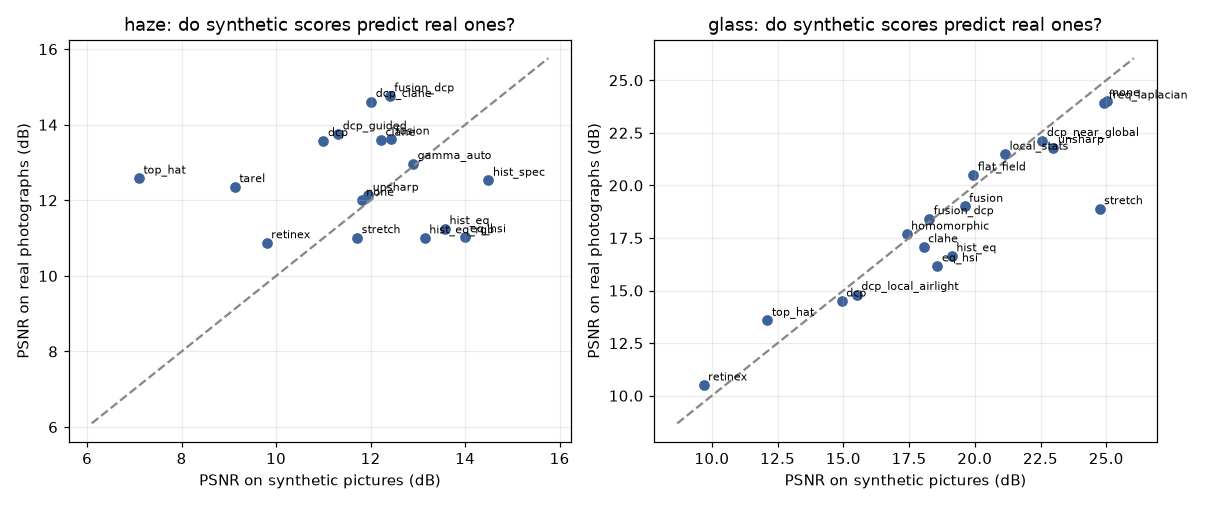
\includegraphics[width=.9\textwidth]{report_synthetic_vs_real.png}\caption{Synthetic against real performance per method.}\end{figure}
\begin{table}[H]\centering\scriptsize\tablein{model_validation}\caption{Fitting the haze model to real pairs: the fitted airlight is 0.60--0.70 (ours was 0.92); the fit with a per-picture affine map is far better than the ramp.}\end{table}
\begin{figure}[H]\centering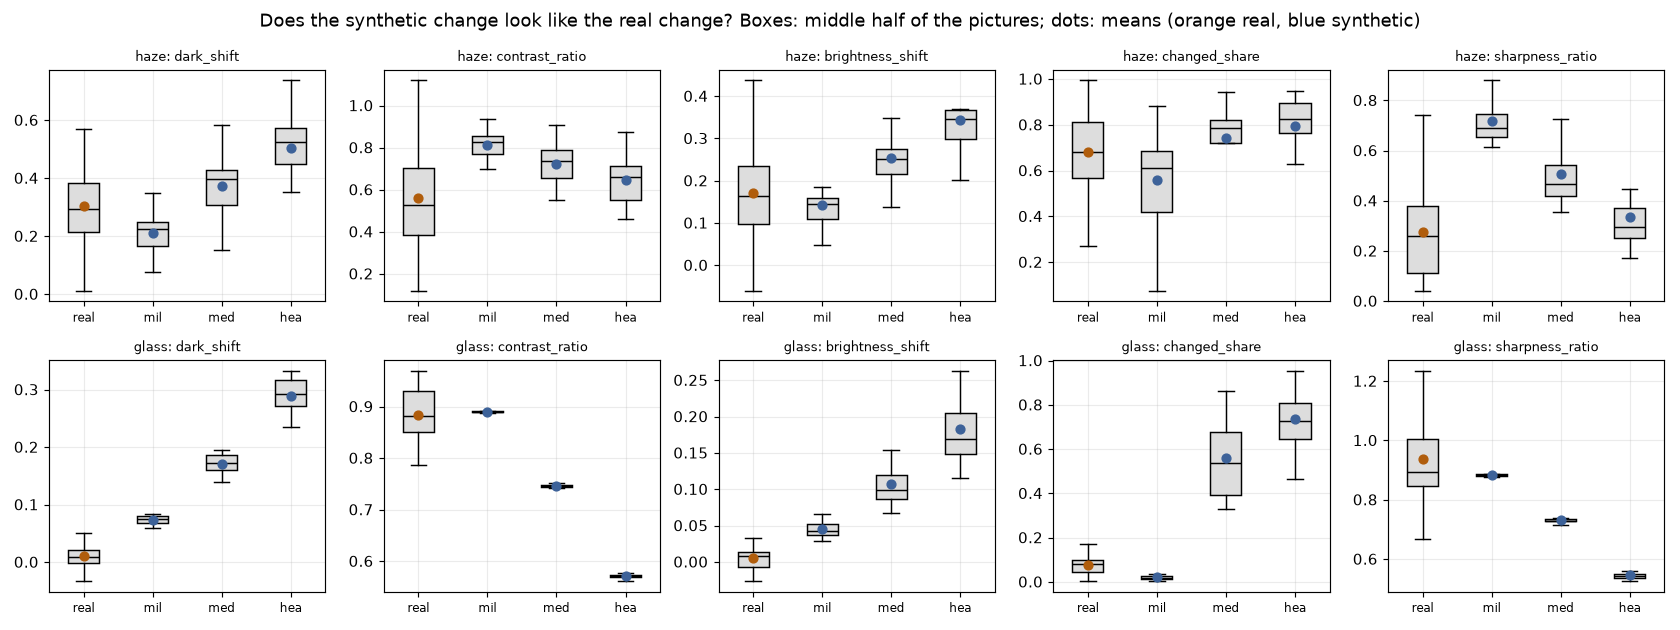
\includegraphics[width=.49\textwidth]{model_signature.png}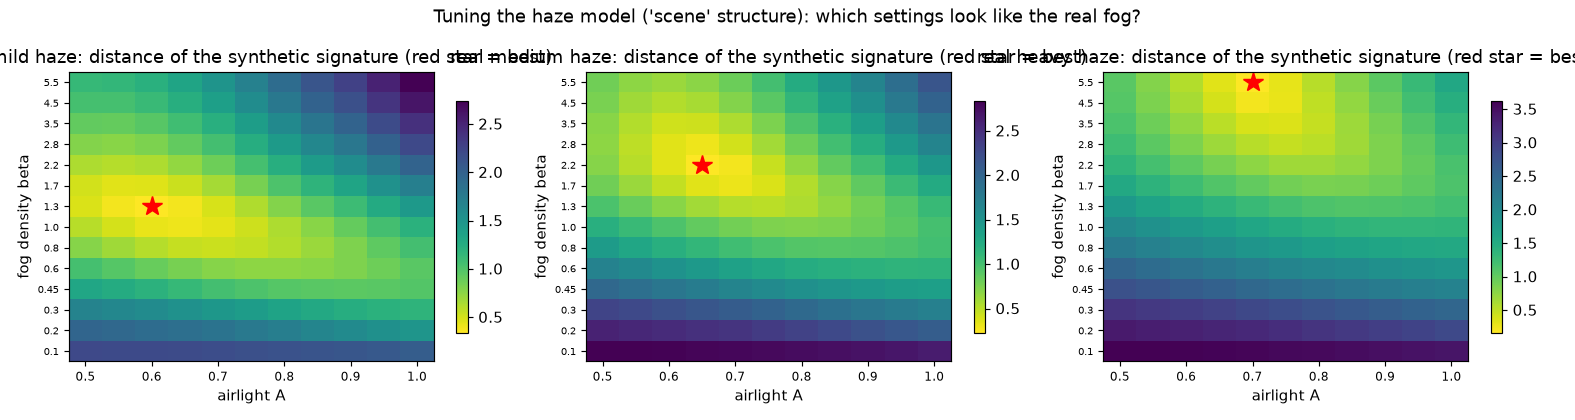
\includegraphics[width=.49\textwidth]{tuning_haze.png}\caption{Left: signature of real against synthetic degradation. Right: tuning sweep for haze presets.}\end{figure}
\begin{table}[H]\centering\scriptsize\tablein{scene_matched}\caption{Same-scene test: each real pair against a synthetic twin of its clear picture. Rankings agree (haze +0.81, glass +0.99), so the earlier mismatch was scene content, not model failure.}\end{table}
\begin{figure}[H]\centering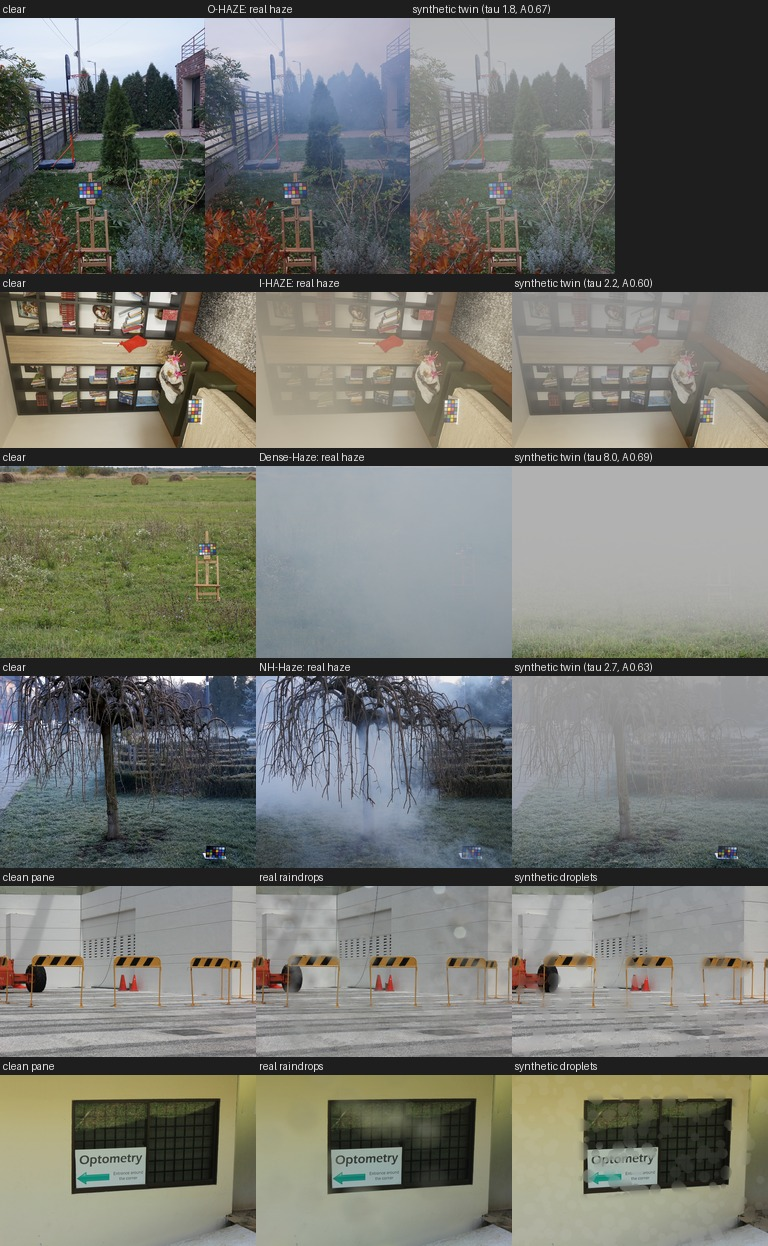
\includegraphics[width=.95\textwidth]{scene_matched_examples.jpg}\caption{Clear picture, real degradation and synthetic twin.}\end{figure}

\subsection{Before and after calibrating the presets}\label{sec:ba}
The original presets were chosen by hand. Calibration fitted haze and glass to real pictures: haze with scene depth, airlight 0.60--0.70 (was 0.92) and denser fog; glass as raindrops only. Water and plastic have no real data and are unchanged, and their results are identical in both runs (a check that the rerun is clean).
\begin{table}[H]\centering\scriptsize\tablein{before_after_presets}\caption{The same experiments with original and calibrated presets. Rank agreement is the Spearman correlation between method rankings on synthetic and real data over 17 methods.}\end{table}
\textbf{What changed.} (1) The original haze flattered DCP (+5.1 dB over nothing); the calibrated haze leaves DCP near doing nothing and favours histogram methods, as real haze does. (2) The original glass made a plain stretch look excellent (+10 dB); on raindrops nothing beats doing nothing, as on real raindrops (agreement 0.53 to 0.92). (3) \textbf{Haze rank agreement fell} (0.53 to 0.09): the best-method verdict moved towards the real one but the full ordering did not. The calibrated haze uses indoor scenes, and the same-scene test (real picture against its synthetic twin) gave +0.81, so scene content is the likely cause, untested. The calibrated haze should not be called a better predictor of the whole ranking.

\subsection{Frequency-domain study and haze removal by subtraction}
\begin{figure}[H]\centering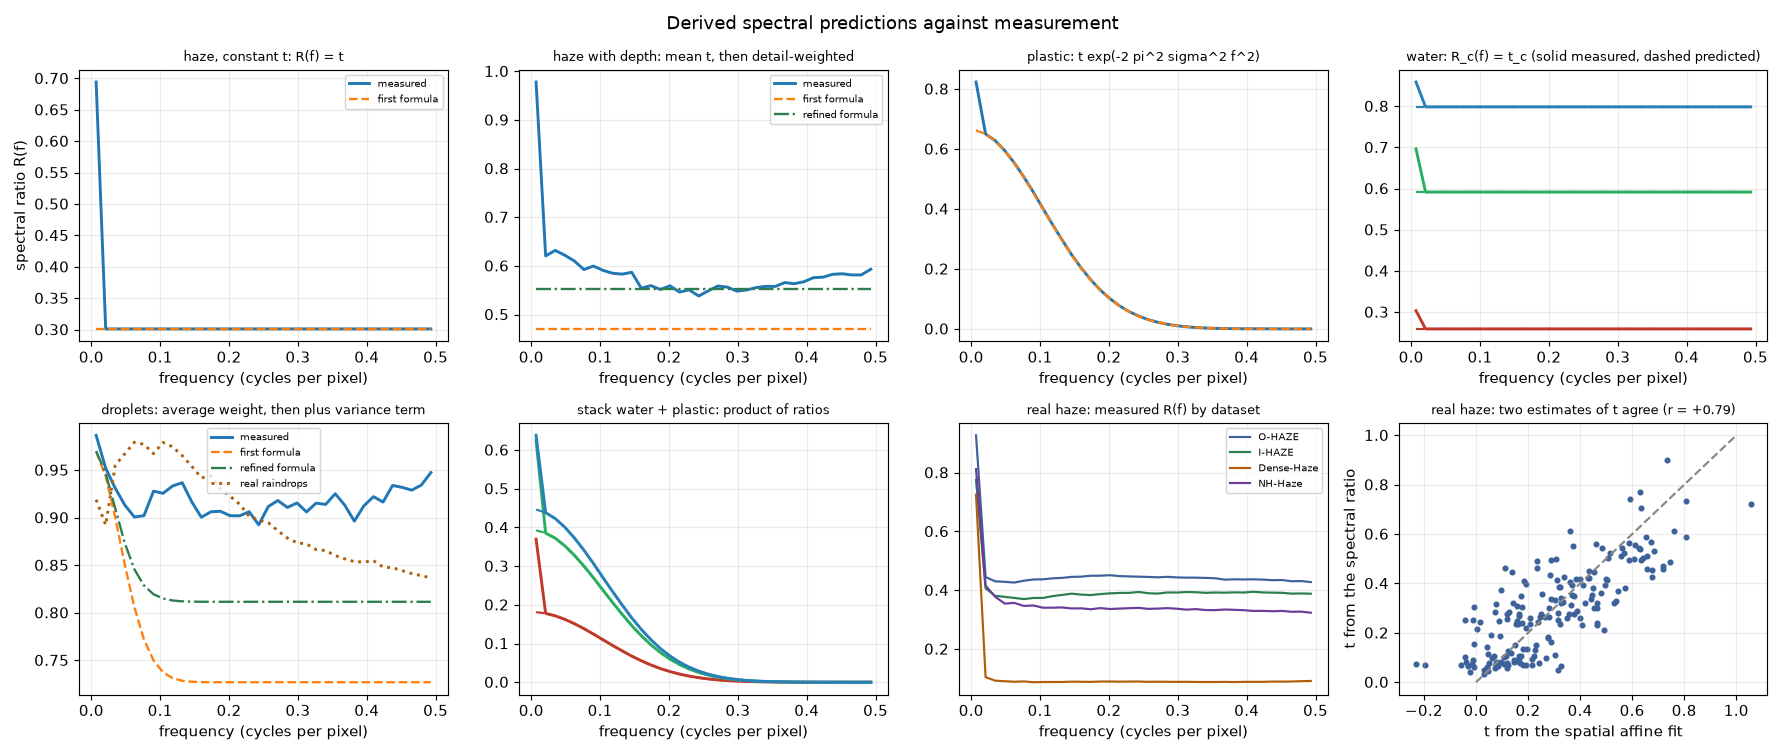
\includegraphics[width=.49\textwidth]{theory_spectral_ratio.png}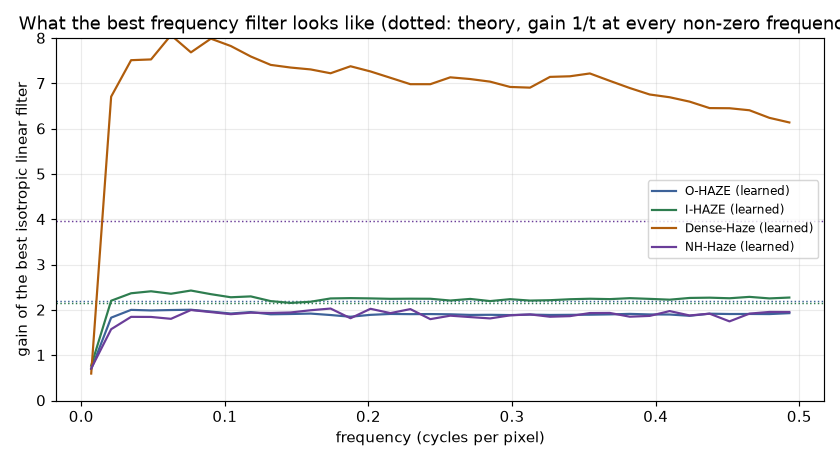
\includegraphics[width=.49\textwidth]{frequency_filter.png}\caption{Left: spectral ratio per medium against theory. Right: oracle radial filter.}\end{figure}
\begin{table}[H]\centering\scriptsize\tablein{frequency_subtraction}\caption{Removing haze by subtraction on held-out real haze pairs. A constant veil fails; a local veil estimated with priors reaches 15.04 dB, above guided DCP (13.85 dB); the best isotropic linear filter (an upper bound) reaches 15.43 dB. The priors came from the same four datasets, so this needs testing elsewhere.}\end{table}
\begin{figure}[H]\centering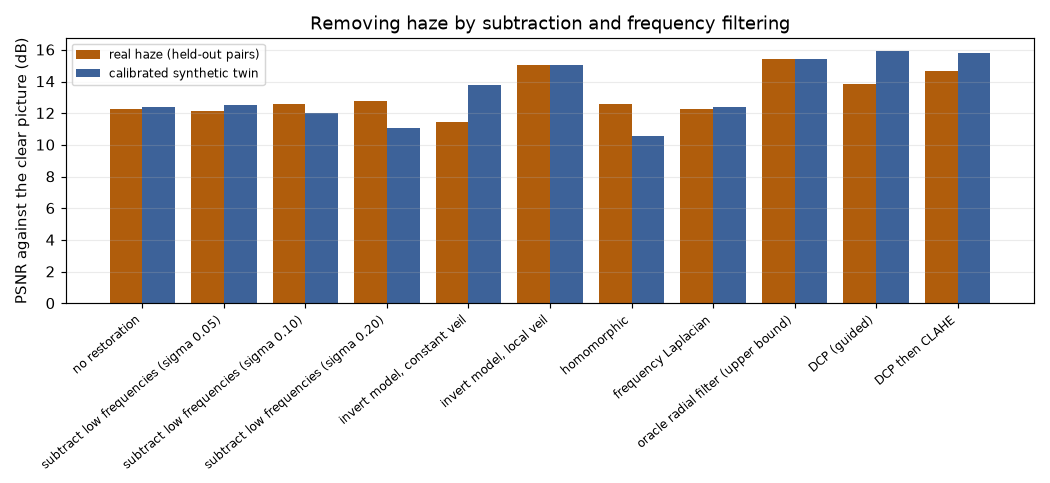
\includegraphics[width=.9\textwidth]{frequency_subtraction.png}\caption{Subtraction methods, before and after.}\end{figure}

\subsection{Failure analysis}
\begin{figure}[H]\centering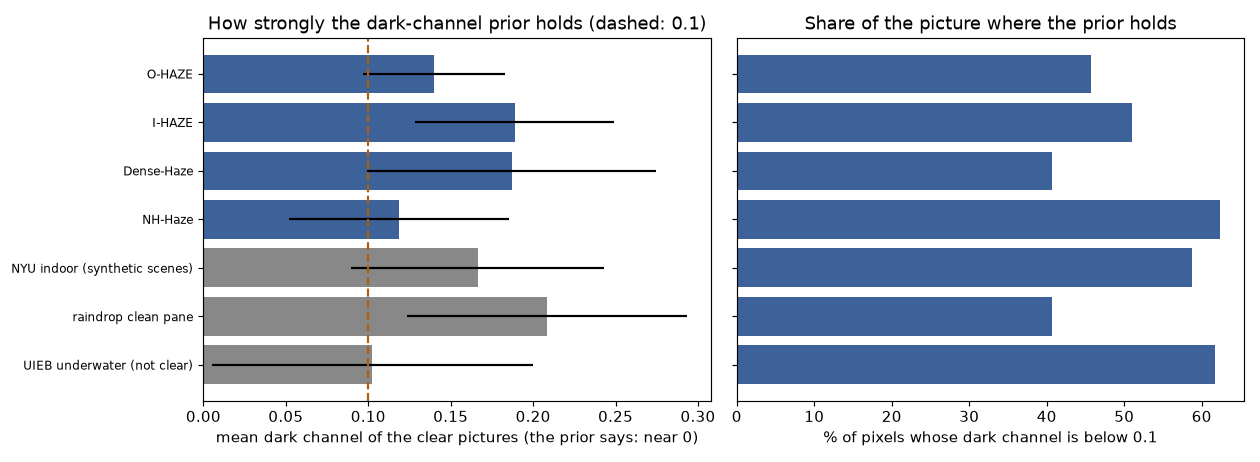
\includegraphics[width=.49\textwidth]{failure_prior_check.png}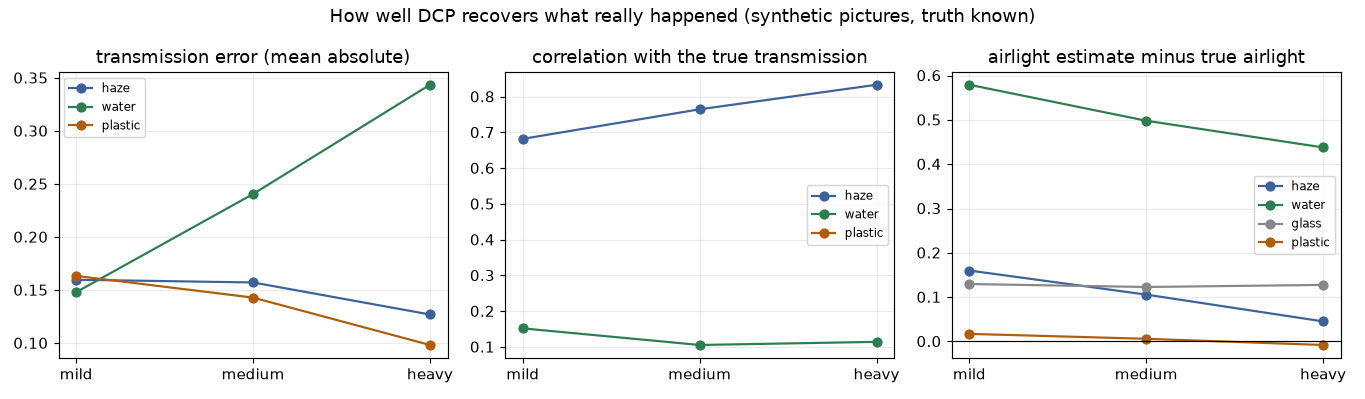
\includegraphics[width=.49\textwidth]{failure_transmission.png}\caption{Dark channel of clear pictures is 0.12--0.21, not 0 (prior holds in 41--62\% of pixels). DCP transmission correlates +0.80 with truth for haze but only +0.11 for water.}\end{figure}
\begin{figure}[H]\centering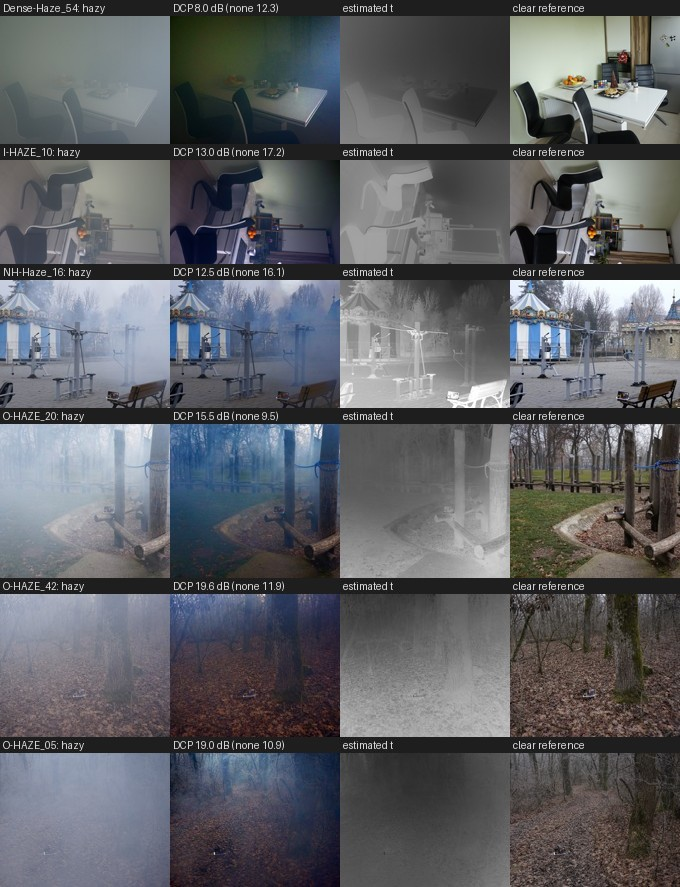
\includegraphics[width=.9\textwidth]{failure_cases_real.jpg}\caption{Failure cases on real pictures.}\end{figure}

\subsection{Stacked media}
\begin{figure}[H]\centering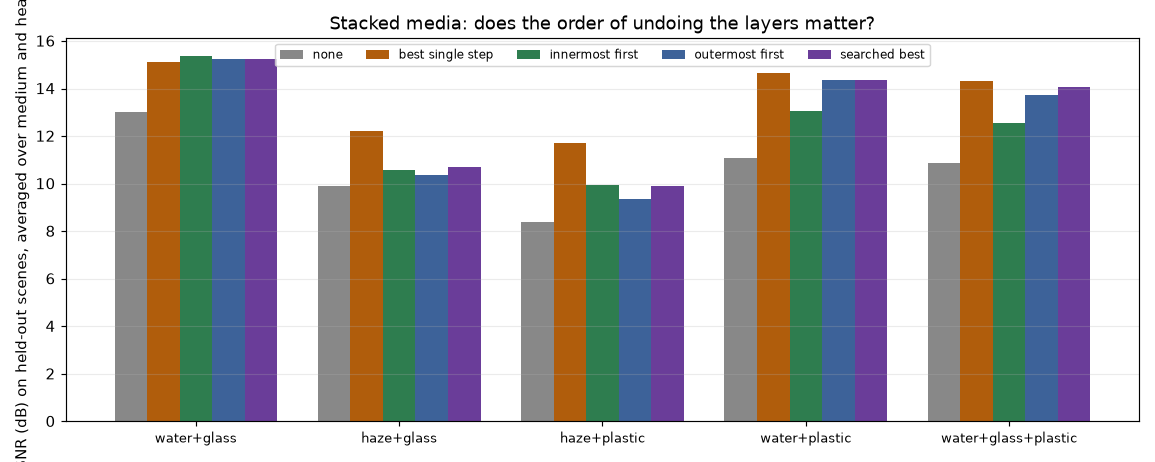
\includegraphics[width=.9\textwidth]{stacked_summary.png}\caption{Calibrated run: the order of undoing layers matters little and not consistently (water+glass 15.24 outermost-first against 15.35 innermost-first; haze+plastic 9.34 against 9.96). The earlier advantage of outermost-first for water stacks relied on the original glass veil.}\end{figure}
\begin{figure}[H]\centering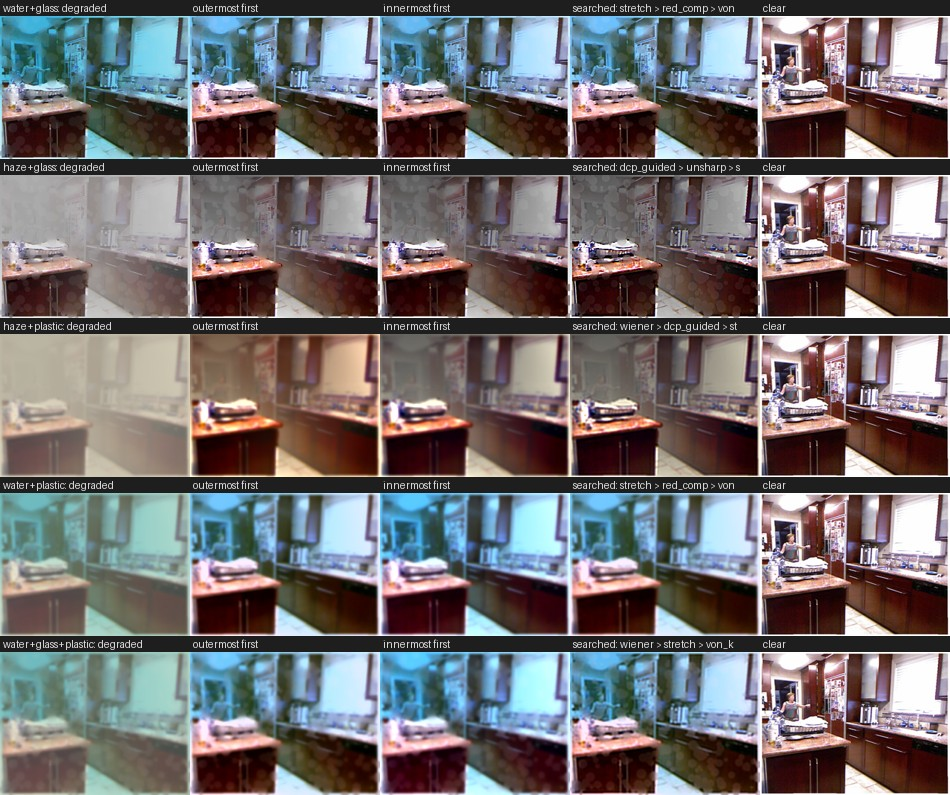
\includegraphics[width=.9\textwidth]{stacked_examples.jpg}\caption{Stacked examples.}\end{figure}

\section{Discussion and limitations}
\begin{itemize}
\item DCP is the right tool for haze only: its prior (dark pixels) and bright-airlight assumption do not hold for water (airlight error 0.50) or plastic. On calibrated and on real haze it is weak, and a contrast step helps.
\item Water: colour correction (red compensation, von Kries) wins \emph{on synthetic water that follows the model it undoes}; real underwater references are missing, so this is a model-favoured result.
\item Contrast stretch wins on veil-style synthetic glass and on plastic because those are affine maps; it cannot help raindrops (a masked blend), and with the calibrated droplets-only glass nothing beats doing nothing.
\item Real haze: DCP$\to$CLAHE is the best simple chain; a locally estimated veil subtraction is competitive (15.04 dB) but its priors are fitted on the same datasets.
\item Open: own captures (water, glass fog/dirt, plastic, stacks), adopting calibrated presets, a separate backscatter coefficient for water, wider sweeps where the best value sat at the grid edge.
\end{itemize}

\section{Reproducibility}
Stage-wise, resumable runs with at most 16 workers (hard ceiling 20) and a 16~GB memory budget: \texttt{run\_stages.py}. A full experiment run takes about 440~s; a benchmark gave 59~s serial against 9~s with 16 workers (6.6$\times$). Every finding, problem and negative result is in \texttt{log.md} (F1--F52).
\end{document}
